\chapter[Risk Modelling for Insurance Groups]{Non-life risk modelling for Insurance Groups}
\label{chap:multiCompany}

The ``Multi Company Model'' is an extension of the \PODRA{} model: It consists of the same components and hence may serve the same purposes for risk modelling of non-life business of direct insurers; its main qualification however is to picture the activities of a group of insurance companies, culminating in an additional component that allows for the assignment of the modelled technical structure to the predefined business structure. The motivation for providing the extended group model with \RA{} goes back to statutory requirements pertaining to group solvency in addition to the regulatory provisions to which the individual insurance company must comply, and also from a different point of view namely neither a solo approach or nor a consolidated approach.
For a more detailed discussion of group modeling and related references we point to Chapter~\ref{chap:insuranceGroup}.

\section*{Parametrization}

In a first step, we open the application and select the \term{MultiCompany} model\footnote{The model has to be enabled in the \ConfigGroovy{} file by adding it to the list of configuration variable {\em models} Add \term{multicompany} and restart \RA.}\todo{}{Where is the description for editing the Config.groovy file?}. The steps for creating a new parametrization correspond to the outline in Chapter~\ref{chap:podra}, for the sake of convenience however we recapitulate the procedure.
 Within the parametrization menu there are two tested examples called \term{Three Companies} and \term{LE-CRTI} (\textbf{l}egal \textbf{e}ntities and their \textbf{c}apital and \textbf{r}isk \textbf{t}ransfer \textbf{i}nstruments). that may be used for analysis purposes with or without changing/modifying/extending the default input parameters. As outlined for \PODRA{}, you may either create a new parametrization or import a .groovy parameter file by right-clicking on \term{Parameterization} and selecting the operation from the context menu.
The newly created (or any other) parametrization is opened by left double-clicking on it or, as a second possibility, right-clicking and selecting the \term{Open} function in the context menu.
\begin{figure}[htb]
	\centering
		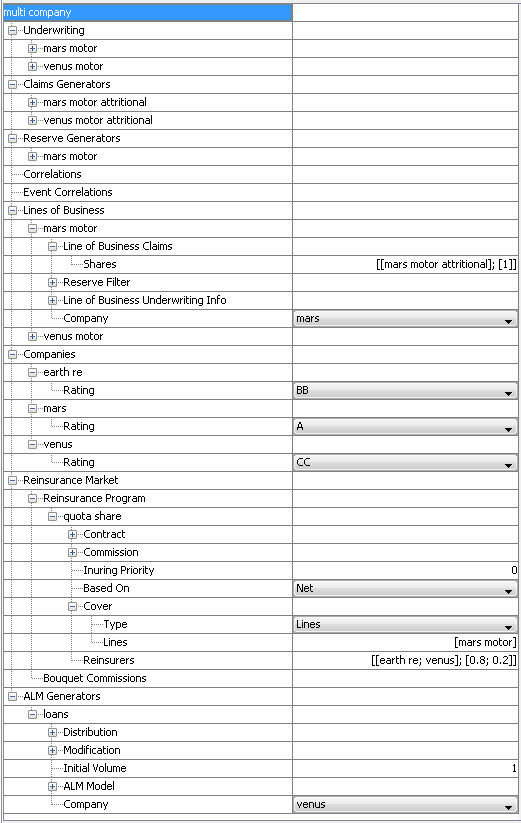
\includegraphics[scale=0.7]{images/multiCompanyEx.png}
	\caption{Multi Company Model}
	\label{fig:multiCompany}
\end{figure}

At this stage the model pops up in the right panel listing all the components coming with the model, compare Figure~\ref{fig:multiCompany}.
The model is similar to \PODRA{} with slight extensions in the components \term{Lines of Business},  \term{Reinsurance Market} (corresponding to \term{Reinsurance} in \PODRA), and \term{ALM Generators}
that are related to the additional component \term{Companies}; altogether turning \PODRA{} into a model suited for the analysis of group risks.
Next, we shortly introduce the new component and outline the resulting modifications for
the components already known from \PODRA.

\paragraph{New component \term{Companies}.}
This component allows to feed into the model a group of contractual partners of the business lines under consideration.
A new company segment is added by right click on \term{Companies}, selecting the button \term{Add} and entering the
name of the (new) insurance company into the pop-up window. Alternatively, an existing company may be duplicated under a new name by right
click and selecting the button \term{Duplicate}.

As illustrated in Figure~\ref{fig:multiCompany} within the company segment, an insurance rating value\footnote{At present the selected value has no impact on the simulation results.} may
be selected for each company from a list with range between \textbf{AAA} and \textbf{D} and default value \textbf{No Default}.


\paragraph{Modified component \term{Lines of Business}.}
As in \PODRA{} we here define the business classes and relate them to the previously specified components \term{Underwriting}, \term{Claims Generators} and \term{Reserve Generators}. In contrast to \PODRA{} the single segments show an additional parameter \term{Company} allowing to attach to the dedicated line of business
the associated insurance company by selection from the list of predefined companies.\footnote{Note that the lines must be related to a predefined company unless the component \term{Companies} is kept empty, in which case \term{MultiCompany} is identical to \PODRA}.
Note that the whole purpose of \term{Lines of Business} is to manage information that is obtained from other components, in other words, the information from other components is sent to the segments of \term{Lines of Business}, filtered according to appropriately defined rules and re-dispatched to the \term{Reinsurance Market} or/and result descriptors.

\paragraph{Modified component \term{ALM Generators}.}
The component \term{ALM Generators} is extended in the same way as \term{Lines of Business}:
The associated company must be attached to the dedicated ALM segment by selection from the list of predefined companies.

\paragraph{Modified component \term{Reinsurance}/\term{Reinsurance Market}.}
Expectedly, segments of \term{Reinsurance Market} distinguish from segments of \term{Reinsurance} in \PODRA{} by an additional parameter \term{Reinsurers}. Here, the selection of one of the predefined companies is optional in contrast to the two aforementioned components. Moreover,
 as reinsurance treaties may be shared between multiple reinsurers, the user may enter as many companies as he wants (sensibly up to the number of insurances in component \term{Companies}) together with the signed share of the treaty. As usual, this kind of parameter may be filled by double-clicking in the cell attached to \term{Reinsurers}.

\section*{Result configuration}
Due to performance and disk space reasons not all possible result variables are generated and stored during a simulation run. Analogous to \PODRA{}, within the ``Multi Company Model'' several result configurations can be defined. By opening a result descriptor
(there is one predefined template named  \term{Aggregate Overview 3}, right click on it and select open) a tree view with the available output variables is shown in the right pane. On each output variable a collection type can be selected. For a more detailed overview of various result descriptors we refer the reader to Chapter~\ref{chap:riskAnalyticsApplication}. Results that are specifically shown for the various company segments are described in full detail in Chapter~\ref{chap:insuranceGroup}.


\section*{Simulation/Evaluation}
Simulations are started by right clicking on \term{Parameterization} or \term{Result templates}. Selecting \term{start simulation} in the appearing context menu the simulation window opens in the right panel. After selecting the dedicated parametrization, result template and number of iterations the simulation run can be started.

Open the result set to see which variables have been generated. On the result variables different risk measures can be added by pressing the appropriate buttons. The options for evaluations include expected value, standard deviation, value at risk and tail value at risk for a given level of \note{check, please}{security}. Any branch of the result tree can be copied to the clipboard by selecting the top left cell of the branch and pressing Ctrl-c.

If the model has been evaluated more than once, with different parameters, the corresponding result sets can be viewed side-by-side using the \term{compare} feature 
selectable in the tree view. Deviations in all result variables can be shown in absolute and relative form. Sensitivity tests of parameters can be done easily using this feature; see Section~\ref{sec:riskAnalyticsResults}.\todo{}{Adjustment of bold font for terms in Parametrization.}


